\documentclass[11pt, conference]{IEEEtran}
\usepackage[spanish]{babel}
\usepackage[utf8]{inputenc}
\usepackage{amsmath}
\usepackage{amsfonts}
\usepackage{cite}
\usepackage{graphicx}

\begin{document}
\title{\bf Algoritmos de Criptografía}
\author{Angel Cutipa Samayani \\
	Jose David Mamani Vilca\\
	Luis Fernando Ttito Surco\\
	Percy Maldonado Quispe \\
	Kevin Jhomar Sanchez Sanchez \\
	}

\onecolumn
\maketitle

\begin{figure}[h]
	\centering
	
\includegraphics[scale=0.6]{ucsp.png}
\end{figure}
\bigskip\bigskip\bigskip\bigskip\bigskip
\bigskip\bigskip\bigskip\bigskip\bigskip

\section{Introducción}
\begin{center}
Hoy en día la seguridad se a transformado en un elemento vital del sector \\ tecnológico,  debido a ello nos introduciremos al mundo de la criptografía para \\ analizar todos los métodos y clases del mismo.

\

Seguiremos a la criptografía atraves de la historia y también veremos como \\ este a repercutido en la vida social de las personas.
\end{center}
\twocolumn

\pagebreak 

\tableofcontents 

\bigskip\bigskip\bigskip\bigskip\bigskip
\bigskip\bigskip\bigskip\bigskip

\pagebreak

\section{¿Qué es la criptografía?}
La Criptografía es una rama de las matemáticas que, al orientarse al mundo de los mensajes digitales, proporciona las herramientas idóneas para solucionar los problemas relacionados con la autenticidad y la confiabilidad. El problema de la confidencialidad se vincula comúnmente con técnicas denominadas de "encripción" y la autenticidad con técnicas denominadas de "firma digital", aunque la solución de ambos, en realidad, se reduce a la aplicación de procedimientos criptográficos de encripción y desencripción.\cite{c}

\

El uso de técnicas criptográficas tiene como propósito prevenir algunas faltas de seguridad en un sistema computarizado.

\

La seguridad, en general, se considera como un aspecto de gran importancia en cualquier corporación que trabaje con sistemas computarizados. El hecho de que gran parte de actividades humanas sean cada vez más dependientes de los sistemas computarizados, hace que la seguridad desempeñe una función protagónica.\cite{d}

\

Las principales características que un sistema de seguridad quiere obtener son:

	\begin{enumerate}
		\item \textbf{Confidencialidad}. Consiste en garantizar que sólo las personas autorizadas tienen acceso a la información.
		\item \textbf{Integridad}. Consiste en garantizar que el documento original no ha sido modificado. El documento puede ser tanto público como confidencial.
		\item \textbf{Autenticación}. Permite garantizar la identidad del autor de la información. 
	\end{enumerate}

\section{Clases Criptografía}
\subsection{Transposición}
Consiste en crear el texto cifrado simplemente desordenando las unidades que forman el texto original; los algoritmos de transposición, reordenan las letras pero no las disfrazan.

\

Ejemplo:
TU SECRETO ES TU PRISIONERO; SI LO SUELTAS, TU ERES
SU PRISIONERO

\begin{figure}[h]
	\begin{center}
		
\includegraphics[scale=0.7]{1.jpg}
		\caption{Representación gráfica de Transposición} 
	\end{center}
\end{figure}
\pagebreak

\subsection{Sustitución}
Consiste en sustituir las unidades del texto original por otras; Los algoritmos de sustitución y los códigos, preservan el orden de los símbolos en claro, pero los disfrazan.

\

Ejemplo de sustitución:\\
ENCONTREMONOS A MEDIANOCHE


\begin{figure}[h]
	\begin{center}
		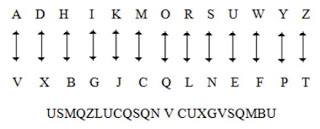
\includegraphics[scale=0.7]{2.jpg}
		\caption{Representación gráfica de Sustitución} 
	\end{center}
\end{figure}

\subsection{Simétrica}
Es un método criptográfico en el cual se usa una misma clave para cifrar y descifrar mensajes en el emisor y el receptor. Las dos partes que se comunican han de ponerse de acuerdo de antemano sobre la clave a usar. Una vez que ambas partes tienen acceso a esta clave, el remitente cifra un mensaje usando la clave, lo envía al destinatario, y éste lo descifra con la misma clave.\cite{e}

\begin{figure}[h]
	\begin{center}
		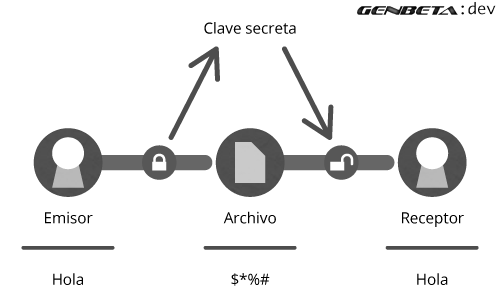
\includegraphics[scale=0.35]{clasico.png}
		\caption{Representación gráfica de la criptografía Simétrica} 
	\end{center}
\end{figure}
\subsubsection{Cifrados de flujo}. cifran el mensaje con correspondencias bit a bit sobre el flujo (stream). Algunos cifrados de flujo son RC4 o RC6.

\subsubsection{Cifrados de Bloque}. cifran el mensaje dividiendo el flujo en bloques de k bits. Cada bloque se corresponde con otro diferente. 

\

Por ejemplo, un bloque con k=3 "010" se podría corresponder con "110". Un ejemplo de cifrado de bloque es el algoritmo AES (que veremos mas adelante).

\subsection{Asimétrica}
La criptografía asimétrica es el método criptográfico que usa un par de claves para el envío de mensajes. Las dos claves pertenecen a la misma persona a la que se ha enviado el mensaje. Una clave es pública y se puede entregar a cualquier persona, la otra clave es privada y el propietario debe guardarla de modo que nadie tenga acceso a ella. Además, los métodos criptográficos garantizan que esa pareja de claves sólo se puede generar una vez, de modo que se puede asumir que no es posible que dos personas hayan obtenido casualmente la misma pareja de claves.

\

Si el remitente usa la clave pública del destinatario para cifrar el mensaje, una vez cifrado, sólo la clave privada del destinatario podrá descifrar este mensaje, ya que es el único que la conoce. Por tanto se logra la confidencialidad del envío del mensaje, nadie salvo el destinatario puede descifrarlo.\cite{f}

\

Si el propietario del par de claves usa su clave privada para cifrar el mensaje, cualquiera puede descifrarlo utilizando su clave pública. En este caso se consigue por tanto la identificación y autentificación del remitente, ya que se sabe que sólo pudo haber sido él quien empleó su clave privada (salvo que alguien se la hubiese podido robar). Esta idea es el fundamento de la firma electrónica.


\begin{figure}[h]
	\begin{center}
		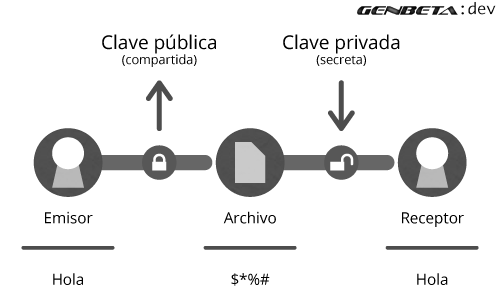
\includegraphics[scale=0.35]{moderno.png}
		\caption{Representación gráfica de la criptografía asimétrica} 
	\end{center}
\end{figure}

\

Los sistemas de cifrado de clave pública o sistemas de cifrado asimétricos se inventaron con el fin de evitar por completo el problema del intercambio de claves de los sistemas de cifrado simétricos. Con las claves públicas no es necesario que el remitente y el destinatario se pongan de acuerdo en la clave a emplear. Todo lo que se requiere es que, antes de iniciar la comunicación secreta, el remitente consiga una copia de la clave pública del destinatario. Es más, esa misma clave pública puede ser usada por cualquiera que desee comunicarse con su propietario. Por tanto, se necesitarán sólo n pares de claves por cada n personas que deseen comunicarse entre sí.

\section{Limitaciones de la Criptografía}


Los algoritmos criptográficos tienden a degradarse con el tiempo (esto hace que sean muy limitados). A medida que transcurre el tiempo, los algoritmos de encriptación se hacen más fáciles de quebrar debido al avance de la velocidad y potencia de los equipos de computación. 

\

Todos los algoritmos criptográficos son vulnerables a los ataques de fuerza bruta (tratar sistemáticamente con cada posible clave de encripción, buscando colisiones para funciones hash, factorizando grandes números, etc.), la fuerza bruta es más fácil de aplicar en la medida que pasa el tiempo.

\

El ejemplo mas claro de la limitación de la criptografía sería:

\

"En 1977 Martin Gardner escribió que los números de 129 dígitos nunca serían factorizados, en 1994 se factorizó uno de esos números"

\

Además de la fuerza bruta, avanzan las matemáticas fundamentales que proveen nuevos métodos y técnicas de criptoanálisis.

\section{Resumen Histórico}
La historia de la criptografía es larga y está llena de anécdotas. Ya las primeras civilizaciones desarrollaron técnicas para enviar mensajes durante las campañas militares de forma que si el mensajero era interceptado la información que portaba no corriera el peligro de caer en manos del enemigo. Posiblemente, el primer criptosistema que se conoce fuera documentado por el historiador griego Polibio: un sistema de sustitución basado en la posición de las letras en una tabla. 

\

También los romanos utilizaron sistemas de sustitución, siendo el método actualmente conocido como César, porque supuestamente Julio César lo utilizó en sus campañas, uno de los más conocidos en la literatura – según algunos autores, en realidad Julio César no utilizaba este sistema de sustitución, pero la atribución tiene tanto arraigo que el nombre de éste método de sustitución ha quedado para los anales de la historia –. 

\

Otro de los métodos criptográficos utilizados por los griegos fue la escitala espartana, un método de transposición basado en un cilindro que servía como clave en el que se enrollaba el mensaje para poder cifrar y descifrar. En 1465 el italiano Leon Battista Alberti inventó un nuevo sistema de sustitución polialfabética que supuso un gran avance de la época. 

\

Otro de los criptógrafos más importantes del siglo XVI fue el francés Blaise de Vigenere que escribió un importante tratado sobre "la escritura secreta" y que diseñó un algoritmo que ha llegado a nuestros días asociado a su nombre. 

\

A Selenus se le debe la obra criptográfica "Cryptomenytices et Cryptographiae" (Lüneburg, 1624). Durante los siglos XVII, XVIII y XIX, el interés de los monarcas por la criptografía fue notable. Las huestes de Felipe II utilizaron durante mucho tiempo un algoritmo con un alfabeto de más de 500 símbolos que los matemáticos del rey consideraban inexpugnable. Cuando el matemático francés François Viète consiguió cripto-analizar aquel sistema para el rey de Francia, a la sazón Enrique IV, el conocimiento mostrado por el rey francés impulsó una queja de la corte española ante del papa Pío V acusando a Enrique IV de utilizar magia negra para vencer a sus ejércitos. Por su parte, la reina María Estuardo, reina de los Escoceses, fue ejecutada por su prima Isabel I de Inglaterra al descubrirse un complot de aquella tras un criptoanálisis exitoso por parte de los matemáticos de Isabel. 

\

Desde el siglo XIX y hasta la Segunda Guerra Mundial las figuras más importantes fueron la del holandés Auguste Kerckhoffs y la del prusiano Friedrich Kasiski. Pero es en el siglo XX cuando la historia de la criptografía vuelve a presentar importantes avances. En especial durante las dos contiendas bélicas que marcaron al siglo: la Gran Guerra y la Segunda Guerra Mundial. A partir del siglo XX, la criptografía usa una nueva herramienta que permitirá conseguir mejores y más seguras cifras: las máquinas de cálculo. La más conocida de las máquinas de cifrado, posiblemente sea la máquina alemana Enigma: una máquina de rotores que automatizaba considerablemente los cálculos que era necesario realizar para las operaciones de cifrado y descifrado de mensajes. Para vencer al ingenio alemán, fue necesario el concurso de los mejores matemáticos de la época y un gran esfuerzo computacional. No en vano, los mayores avances tanto en el campo de la criptografía como en el del cripto-análisis no empezaron hasta entonces. 

\

Tras la conclusión de la Segunda Guerra Mundial, la criptografía tiene un desarrollo teórico importante; siendo Claude Shannon y sus investigaciones sobre teoría de la información esenciales hitos en dicho desarrollo. Además, los avances en computación automática suponen tanto una amenaza para los sistemas existentes como una oportunidad para el desarrollo de nuevos sistemas.

\

A mediados de los años 70 el Departamento de Normas y Estándares norteamericano publica el primer diseño lógico de un cifrador que estaría llamado a ser el principal sistema criptográfico de finales de siglo: el Estándar de Cifrado de Datos o DES. En esas mismas fechas ya se empezaba a gestar lo que sería la, hasta ahora, última revolución de la criptografía teórica y práctica: los sistemas asimétricos. Estos sistemas supusieron un salto cualitativo importante ya que permitieron introducir la criptografía en otros campos que hoy día son esenciales, como el de la firma digital.

\section{Criptografía Clásica}
\subsection{Concepto}
Como ya hemos visto, la criptografía es casi tan antigua como las primeras civilizaciones de nuestro planeta. Ya en el siglo V antes de J.C. se usaban técnicas de cifrado para proteger a la información. Se pretendía garantizar sólo la confidencialidad y la autenticidad de los mensajes.

La criptografía clásica abarca desde tiempos inmemoriales hasta la mitad del siglo XX. El punto de inflexión en esta clasificación la marcan tres hechos relevantes:
	\begin{enumerate}
		\item  En el año 1948 se publica el estudio de Claude Shannon sobre la Teoría de la Información.
		\item  En 1974 aparece el estándar de cifra DES.
		\item  En el año 1976 se publica el estudio realizado por W. Diffie y M. Hellman sobre la aplicación de funciones matemáticas de un solo sentido a un modelo de cifra, denominado cifrado con clave pública.
	\end{enumerate}
\subsection{Algoritmos} 
\subsubsection{Transposición Inversa}
Es nuestro algoritmo más simple. Lo requerido para poder ejecutar el algoritmo, se debe saber donde inicia y donde termina nuestro mensaje. Se trata de invertir el inicio y el final de nuestro mensaje, cabe destacar que el algoritmo de cifrado es igual al de descifrado. 
\
Ejemplo: 
\\
$
Mensaje: hola mundo\\ 
Cripto: odnumaloh \\
$


Este texto tiene adjunto los algoritmos mencionados programados en JAVA, por lo que se sugiere ver los códigos fuente y probar su funcionamiento. Debido a eso, se procurará no añadir aquí dichos códigos y facilitar así la lectura del documento. Sin embargo se mostraran los diseños de estos programas, en este caso corresponden, diagramas de clase. 
\subsubsection{Transposición Simple}
El algoritmo divide un mensaje en claro símbolo por símbolo, si el número de símbolos es impar, el primer grupo de símbolos tendrá un elemento más. Podemos ver el algoritmo como si numeráramos los elementos, en el primer bloque tendremos los elementos impares mientras en el segundo estarán los elementos pares. Para finalizar concatenamos los bloques y así tendremos el criptograma. 
Ejemplo: \\
$
Mcla: Hola mundo \\
Bloque1: hlmno \\
Bloque2: oaud \\
Cripto: hlmnooaud\\ 
$

El proceso de descifrado, es similar, dividimos el criptograma en dos partes iguales, la primera mitad del criptograma será el primer bloque. Teniendo ambos bloques, se intercalan uno a uno los elementos de cada bloque, puede leerse el ejemplo de abajo hacia arriba, para ver la operación.

\subsubsection{Cesar}
En el siglo I a.d.C., Julio César usa este cifrado, cuyo algoritmo consiste en el desplazamiento de tres espacios hacia la derecha de los caracteres del texto en claro. Es un cifrado por sustitución monoalfabético en el que las operaciones se realizan módulo n, siendo n el número de elementos del alfabeto (en aquel entonces latín).

\begin{figure}[h]
	\begin{center}
		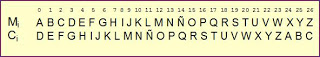
\includegraphics[scale=0.7]{5.jpg}
		\caption{Representacion de Cesar} 
	\end{center}
\end{figure}

Cada letra se cifrará siempre igual. Es una gran debilidad y hace que este sistema sea muy vulnerable y fácil de atacar simplemente usando las estadísticas del lenguaje.

\subsubsection{Escítala}

La escítala era usada en el siglo V a.d.C. por el pueblo griego de los lacedemonios. Consistía en un bastón en el que se enrollaba una cinta de cuero y luego se escribía en ella el mensaje de forma longitudinal. Al desenrollar la cinta, las letras aparecen desordenadas. La única posibilidad de recuperar el texto en claro pasaba por enrollar dicha cinta en un bastón con el mismo diámetro que el usado en el extremo emisor y leer el mensaje de forma longitudinal. La clave del sistema está en el diámetro del bastón. Se trata de una cifra por transposición pues los caracteres del criptograma son los mismos que en el texto en claro distribuidos de otra forma.


\begin{figure}[h]
	\begin{center}
		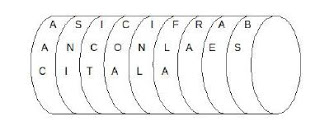
\includegraphics[scale=0.7]{3.jpg}
		\caption{Representación gráfica de Escítala} 
	\end{center}
\end{figure}


\subsubsection{Vigenere}
Es un cifrado basado en diferentes series de caracteres o letras del cifrado César formando estos caracteres una tabla, llamada tabla de Vigenère, que se usa como clave. El cifrado de Vigenère es un cifrado de sustitución simple polialfabético.



\begin{figure}[h]
	\begin{center}
		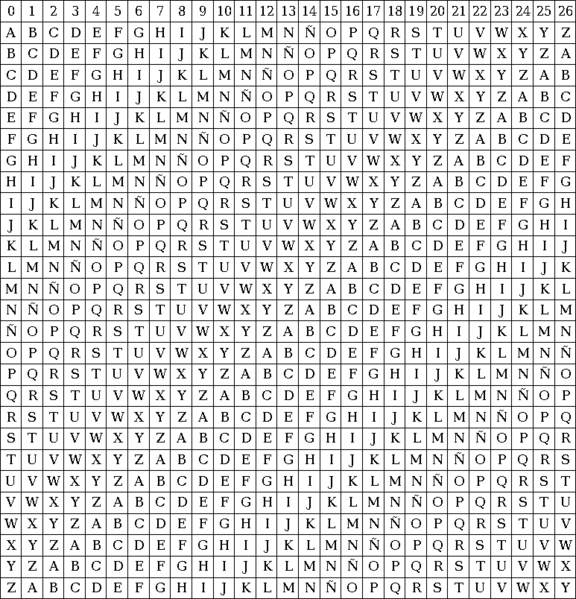
\includegraphics[scale=0.5]{Cuadro_Vigenere.PNG}
		\caption{Cuadro de Vigenere} 
	\end{center}
\end{figure}

El cifrado Vigenère se ha reinventado muchas veces. El método original fue descrito por Giovan Battista Belasso en su libro de 1553 La cifra del Sig. Giovan Battista Belasso. Sin embargo, fue incorrectamente atribuido más tarde a Blaise de Vigenère, concretamente en el siglo XIX, y por ello aún se le conoce como el "cifrado Vigenère".

\

Este cifrado es conocido porque es fácil de entender e implementar, además parece irresoluble; esto le hizo valedor del apodo el código indescifrable (le chiffre indéchiffrable, en francés).

\subsubsection{Vernam}
Se usa el mismo algoritmo para cifrar y para descifrar el mensaje. Usa una clave constituida por una sucesión de símbolos (bits o caracteres), operando XOR cada símbolo de ésta con el correspondiente del texto en claro.

\

 Debido a la definición de la función XOR, el descifrado se realiza, igualmente, operando con dicha función cada bit de la misma serie cifrante con el correspondiente del texto cifrado. Si la serie cifrante no se repite, es aleatoria, y de longitud igual, al menos, al texto a cifrar éste cifrado alcanza el secreto perfecto. Además, es el único que verifica tal condición.
 
 
 \begin{figure}[h]
 	\begin{center}
 		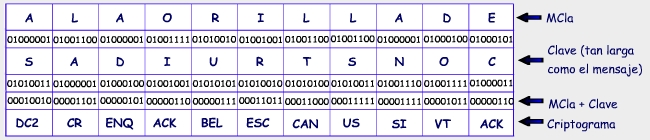
\includegraphics[scale=0.38]{vernam2223.jpg}
 		\caption{Cuadro de Vernam} 
 	\end{center}
 \end{figure}
\subsubsection{Polybios}

Es el cifrado por sustitución de caracteres más antiguo que se conoce (siglo II a.d.C.) pero como duplica el tamaño del texto en claro, con letras o números, resulta poco interesante.
	
	\begin{figure}[h]
		\begin{center}
			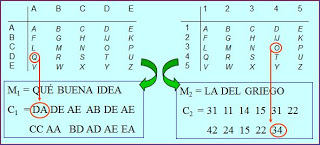
\includegraphics[scale=0.7]{4.jpg}
			\caption{Representacion de Polybios} 
		\end{center}
	\end{figure}	
\pagebreak	
	
\section{Criptografía Moderna}

\subsection{Concepto}

Como hemos visto en el apartado anterior, los sistemas criptográficos clásicos presentaban una dificultad en cuanto a la relación complejidad-longitud de la clave / tiempo necesario para encriptar y desencriptar el mensaje.

\

En la era moderna esta barrera clásica se rompió, debido principalmente a los siguientes factores:

\
\begin{enumerate}
	
	\item \textbf{Velocidad de cálculo}. con la aparición de los computadores se dispuso de una potencia de cálculo muy superior a la de los métodos clásicos.
	
	\item \textbf{Avance de las matemáticas} que permitieron encontrar y definir con claridad sistemas criptográficos estables y seguros.
	
	\item \textbf{Necesidades de seguridad} surgieron muchas actividades nuevas que precisaban la ocultación de datos, con lo que la Criptología experimentó un fuerte avance.
\end{enumerate}

\

A partir de estas bases surgieron nuevos y complejos sistemas criptográficos, que se clasificaron en dos tipos o familias principales, los de clave simétrica y los de clave asimétricos. Los modernos algoritmos de encriptación simétricos mezclan la trasposición y la permutación, mientras que los de clave pública se basan más en complejas operaciones matemáticas.


\subsection{Algoritmos}
\subsubsection{DES}
Data Encryption Standard (DES) es un algoritmo de cifrado, es decir, un método para cifrar información, escogido como FIPS en los Estados Unidos en 1976, y cuyo uso se ha propagado ampliamente por todo el mundo. El algoritmo fue controvertido al principio, con algunos elementos de diseño clasificados, una longitud de clave relativamente corta.\cite{h}

\

Hoy en día, DES se considera inseguro para muchas aplicaciones. Esto se debe principalmente a que el tamaño de clave de 56 bits es corto; las claves de DES se han roto en menos de 24 horas. Existen también resultados analíticos que demuestran debilidades teóricas en su cifrado, aunque son inviables en la práctica. Se cree que el algoritmo es seguro en la práctica en su variante de Triple DES, aunque existan ataques teóricos.

\

Desde hace algunos años, el algoritmo ha sido sustituido por el nuevo AES (Advanced Encryption Standard).

\textbf{La estructura básica del algoritmo}  aparece representada en la Figura 10: hay 16 fases idénticas de proceso, denominadas rondas. También hay una permutación inicial y final denominadas PI y PF, que son funciones inversas entre sí (PI "deshace" la acción de PF, y viceversa). PI y PF no son criptográficamente significativas, pero se incluyeron presuntamente para facilitar la carga y descarga de bloques sobre el hardware de mediados de los 70. Antes de las rondas, el bloque es dividido en dos mitades de 32 bits y procesadas alternativamente. Este entrecruzamiento se conoce como esquema Feistel.

\

La estructura de Feistel asegura que el cifrado y el descifrado sean procesos muy similares — la única diferencia es que las subclaves se aplican en orden inverso cuando desciframos. El resto del algoritmo es idéntico. Esto simplifica enormemente la implementación, en especial sobre hardware, al no haber necesidad de algoritmos distintos para el cifrado y el descifrado.

\

El símbolo rojo  representa la operación OR exclusivo (XOR). La función-F mezcla la mitad del bloque con parte de la clave. La salida de la función-F se combina entonces con la otra mitad del bloque, y los bloques son intercambiados antes de la siguiente ronda. Tras la última ronda, las mitades no se intercambian; ésta es una característica de la estructura de Feistel que hace que el cifrado y el descifrado sean procesos parecidos.


\begin{figure}[h]
	\begin{center}
		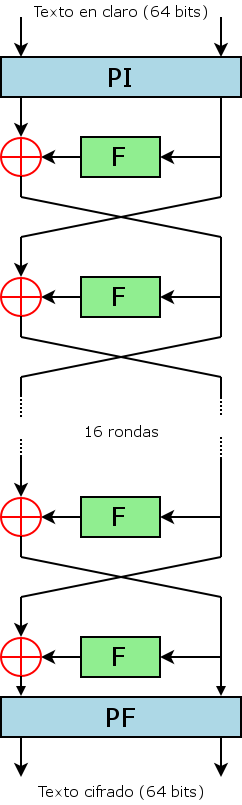
\includegraphics[scale=0.35]{DES-estructura-basica.png}
		\caption{La estructura general de Feistel en DES} 
	\end{center}
\end{figure}

\

\subsubsection{Triple DES}
Se le llama al algoritmo que hace triple cifrado del DES. También es conocido como TDES o 3DES, fue desarrollado por IBM en 1998.

\

Este método de cifrado es inmune al ataque por encuentro a medio camino, doblando la longitud efectiva de la clave (112 bits), pero en cambio es preciso triplicar el número de operaciones de cifrado, haciendo este método de cifrado muchísimo más seguro que el DES. Por tanto, la longitud de la clave usada será de 168 bits (3x56 bits), aunque como se ha dicho su eficacia solo sea de 112 bits. Se continúa cifrando bloques de 64 bits.

\

El Triple DES está desapareciendo lentamente, siendo reemplazado por el algoritmo AES. Sin embargo, la mayoría de las tarjetas de crédito y otros medios de pago electrónicos tienen como estándar el algoritmo Triple DES (anteriormente usaban el DES). Por su diseño, el DES y por lo tanto el TDES son algoritmos lentos. AES puede llegar a ser hasta 6 veces más rápido y a la fecha no se ha encontrado ninguna vulnerabilidad.

\

\subsubsection{MD5}
(Message-Digest Algorithm 5) Es un algoritmo de reducción criptográfico de 128 bits ampliamente usado. uno de sus usos es el de comprobar que algún archivo no haya sido modificado.

\

La codificación del MD5 de 128 bits es representada típicamente como un número de 32 dígitos hexadecimal. El siguiente código de 28 bytes ASCII será tratado con MD5 y veremos su correspondiente hash de salida:

\begin{center}
	$MD5("Generando\ un\ MD5\ de\ un\ texto")$\\ $5df9f63916ebf8528697b629022993e8$
\end{center}
Un pequeño cambio en el texto (cambiar '5' por 'S') produce una salida completamente diferente.
\begin{center}
	$MD5("Generando\ un\ MDS\ de\ un\ texto")$\\ $e14a3ff5b5e67ede599cac94358e1028$
\end{center}
Otro ejemplo serí­a la codificación de un campo vací­o:
\begin{center}
	$MD5("")$\\ $d41d8cd98f00b204e9800998ecf8427e$
\end{center}

\

\subsubsection{Blowfish}
Es un codificador de bloques simétricos, diseñado por Bruce Schneier en 1993 e incluido en un gran número de conjuntos de codificadores y productos de cifrado. No se han encontrado técnicas de criptoanálisis efectivas contra el Blowfish.

\

Blowfish usa bloques de 64 bits y claves que van desde los 32 bits hasta 448 bits. Es un codificador de 16 rondas Feistel y usa llaves que dependen de las Cajas-S. Tiene una estructura similar a CAST-128, el cual usa Cajas-S fijas.

\


\begin{figure}[h]
	\begin{center}
		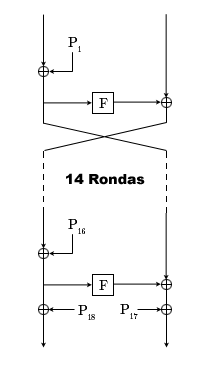
\includegraphics[scale=0.9]{DiagramaBlowfish.png}
		\caption{Diagrama de Blowfish} 
	\end{center}
\end{figure}

El diagrama muestra la acción de Blowfish. Cada línea representa 32 bits. El algoritmo guarda 2 arrays de subclaves: El array P de 18 entradas y 4 cajas-S de 256 entradas. Una entrada del array P es usada cada ronda, después de la ronda final, a cada mitad del bloque de datos se le aplica un XOR con uno de las 2 entradas del array P que no han sido utilizadas.

\

La función divide las entrada de 32 bits en 4 bloques de 8 bits, y usa los bloques como entradas para las cajas-S. Las salidas deben estar en módulo 232 y se les aplica un ok XOR para producir la salida final de 32 bits.

\

Debido a que Blowfish está en la red Feistel, puede ser invertido aplicando un XOR entre P17 y P18 al bloque texto codificado, y así sucesivamente se usan las P-entradas en orden reversivo.

\

La generación de claves comienza inicializando los P-arrays y las cajas-S con los valores derivados de los dígitos hexadecimales de pi, los cuales no contienen patrones obvios. A la clave secreta se le aplica un XOR con las P-entradas en orden (ciclando la clave si es necesario). Un bloque de 64 bits de puros ceros es cifrado con el algoritmo como se indica. El texto codificado resultante reemplaza a P1 y P2. Entonces el texto codificado es cifrado de nuevo con las nuevas subclaves, P3 y P4 son reemplazados por el nuevo texto codificado. Esto continúa, reemplazando todas las entradas del P-array y todas las entradas de las cajas-S. En total, el algoritmo de cifrado Blowfish correrá 521 veces para generar todas las subclaves, cerca de 4KB de datos son procesados.

\bigskip\bigskip\bigskip

\begin{figure}[h]
	\begin{center}
		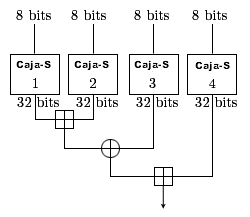
\includegraphics[scale=0.9]{BlowfishFuncionF.png}
		\caption{Diagrama de Blowfish a nivel de bits} 
	\end{center}
\end{figure}

\pagebreak

\subsubsection{RSA}
Es un sistema criptográfico de clave pública desarrollado en 1977 por ingenieros estadounidenses. En la actualidad, RSA es el primer y más utilizado algoritmo de este tipo y es válido tanto para cifrar como para firmar digitalmente.

\

La seguridad de este algoritmo radica en el problema de la factorización de números enteros. Los mensajes enviados se representan mediante números, y el funcionamiento se basa en el producto, conocido, de dos números primos grandes elegidos al azar y mantenidos en secreto. Actualmente estos primos son del orden de 10200, y se prevé que su tamaño aumente con el aumento de la capacidad de cálculo de los ordenadores.

\

Como en todo sistema de clave pública, cada usuario posee dos claves de cifrado: una pública y otra privada. Cuando se quiere enviar un mensaje, el emisor busca la clave pública del receptor, cifra su mensaje con esa clave, y una vez que el mensaje cifrado llega al receptor, este se ocupa de descifrarlo usando su clave privada.

\

La seguridad del criptosistema RSA está basado en dos problemas matemáticos: el problema de factorizar números grandes y el problema RSA. El descifrado completo de un texto cifrado con RSA es computacionalmente intratable, no se ha encontrado un algoritmo eficiente todavía para ambos problemas. Proveyendo la seguridad contra el descifrado parcial podría requerir la adición de una seguridad padding scheme.

\

El problema del RSA se define como la tarea de tomar raíces eth módulo a componer n: recuperando un valor m tal que $me=c\ mod\ n$, donde $(e, n)$ es una clave pública RSA y c es el texto cifrado con RSA. Actualmente la aproximación para solventar el problema del RSA es el factor del módulo n. Con la capacidad para recuperar factores primos, un atacante puede computar el exponente secreto d desde una clave pública $(e, n)$, entonces descifra c usando el procedimiento standard. Para conseguir esto, un atacante factoriza n en p y q, y computa $(p-1)(q-1)$ con lo que le permite determinar d y e. No se ha encontrado ningún método en tiempo polinómico para la factorización de enteros largos. Ver factorización de enteros para la discusión de este problema.

\

La factorización de números grandes por lo general proponen métodos teniendo 663 bits de longitud usando métodos distribuidos avanzados. Las claves RSA son normalmente entre 1024-2048 bits de longitud. Algunos expertos creen que las claves de 1024 bits podrían comenzar a ser débiles en poco tiempo; con claves de 4096 bits podrían ser rotas en un futuro. Por lo tanto, si n es suficientemente grande el algoritmo RSA es seguro. Si n tiene 256 bits o menos, puede ser factorizado en pocas horas con un computador personal, usando software libre. Si n tiene 512 bits o menos, puede ser factorizado por varios cientos de computadoras como en 1999. Un dispositivo hardware teórico llamado TWIRL descrito por Shamir y Tromer en el 2003 cuestionó a la seguridad de claves de 1024 bits. Es actualmente recomendado que n sea como mínimo de 2048 bits de longitud.

\

En 1993, Peter Shor publicó su algoritmo, mostrando que una computadora cuántica podría en principio mejorar la factorización en tiempo polinomial, mostrando RSA como un algoritmo obsoleto. Sin embargo, las computadoras cuánticas no se esperan que acaben su desarrollo hasta dentro de muchos años.

\

\subsubsection{DSA}
(Digital Signature Algorithm) Es un estándar del Gobierno Federal de los Estados Unidos de América o FIPS para firmas digitales. Fue un Algoritmo propuesto por el Instituto Nacional de Normas y Tecnología de los Estados Unidos para su uso en su Estándar de Firma Digital (DSS), especificado en el FIPS 186. DSA se hizo público el 30 de agosto de 1991, este algoritmo como su nombre lo indica, sirve para firmar y no para cifrar información. Una desventaja de este algoritmo es que requiere mucho más tiempo de cómputo que RSA.

\

\textbf{Generación de claves}
\begin{enumerate}
\item Elegir un número primo $p$ de $L$ bits, donde \\$512 \leq L \leq 1024$ y $L$ es divisible por 64.
\item Elegir un número primo q de 160 bits, tal que \\$p-1=qz$, donde $z$ es algún número natural.
\item Elegir $h$, donde $1<h<p-1$ tal que\\ $g=hz(mod\ p)>1$.
\item Elegir $x$ de forma aleatoria, donde $1<x<q-1$.
\item Calcular $~y=gx(mod\ p)$.
\end{enumerate}
Los datos públicos son p, q, g e y. x es la clave privada.

\

\textbf{Firma}
\begin{enumerate}
\item Elegir un número aleatorio $k$, donde $1 < k < q$.
\item Calcular $r = (g^k\ mod\ p)mod\ q$.
\item Calcular $s = k^-1(H(m)+r*x) mod q$, donde $H(m)$ es la función hash SHA-1 aplicada al mensaje $m$.
\item La firma es el par $(r, s)$.
\end{enumerate}
Si r ó s es cero, se vuelve a repetir el procedimiento.

\

\textbf{Verificación}

\begin{enumerate}
\item Calcular $w = (s)^-1(mod\ q)$.
\item Calcular $u1 = H(m)*w(mod\ q)$.
\item Calcular $u2 = r*w(mod\ q)$.
\item Calcular $v = [g^(u1)*^(yu2)mod\ p]\ mod\ q$.
\item La firma es válida si $v = r$.
\end{enumerate}

\

\subsubsection{ElGamal}
Se refiere a un esquema de cifrado basado en el problema matemático del logaritmo discreto. Es un algoritmo de criptografía asimétrica basado en la idea de Diffie-Hellman y que funciona de una forma parecida a este algoritmo discreto.

\

Hasta el momento el algoritmo ElGamal de cifrado/descifrado puede ser considerado un algoritmo efectivo.

\

Un adversario con la habilidad de calcular logaritmos discretos podría ser capaz de romper un cifrado ElGamal. Sin embargo, en la actualidad, el algoritmo de computación de logaritmos discretos (cuando trabajamos módulo un primo) es subexponencial con una complejidad de $\lambda = 1/3$, la misma que la de factorizar dos números primos, y por tanto, no es accesible de realizar tal tarea en números grandes en un tiempo razonable. El logaritmo discreto es aún más difícil si trabajamos en otros grupos (como por ejemplo, curvas elípticas).

\

Mostremos el criptosistema propuesto inicialmente por Tahar ElGamal en su artículo.

\

\textbf{Generación de la clave}

Para generar la clave, Alicia escoge un número primo $p$, cualquiera tal que $p-1$, tenga un factor primo grande (esto se pide para que el problema del logaritmo discreto sea difícil ). Además elige dos números aleatorios $g$, (el generador) y $a$, (que actuará como clave privada) tal que $a\in \{0,\ldots ,p-1\}$ $a\in \{0,\ldots ,p-1\}$.

\

Alicia calcula el valor de $K=\,g^{a}{\pmod {p}}$ $K=\,g^{a}{\pmod {p}}$. La clave pública será $(g,p,K)$ $(g,p,K)$, mientras que el valor de $a$ lo mantendrá en secreto.


\

\textbf{Cifrado}

Supongamos que Bruno tiene un texto claro que quiere enviar cifrado a Alicia. Lo primero por hacer es convertir este texto en un entero entre 1 y $p-1$ , obteniendo un $m$, (esto no es parte del cifrado, sino que es una manera de codificar estándar, conocida por todos). Luego Bruno escoge arbitrariamente un número $ b\in \{2,\ldots ,p-1\}$ $b\in \{2,\ldots ,p-1\}$ (que mantendrá secreto) para finalmente calcular:

$y_{1}=g^{b}\,{\pmod {p}}$ $y_{1}=g^{b}\,{\pmod {p}}$
$ y_{2}=K^{b}\,m\,{\pmod {p}}$$y_{2}=K^{b}\,m\,{\pmod {p}}$
El mensaje cifrado final corresponde a la tupla $ \,C_{b}(m,b)=(y_{1},y_{2})$ $ \,C_{b}(m,b)=(y_{1},y_{2})$


\

\textbf{Decifrado}

Para descifrar se tiene que realizar el siguiente cálculo:

\

$y_{1}^{-a}y_{2}{\pmod {p}}$ $ y_{1}^{-a}y_{2}{\pmod {p}}$
donde $ y_{1}^{-a}$ $ y_{1}^{-a}$ representa el inverso de $y_{1}^{a}$ $y_{1}^{a}$ módulo $p$ (que, utilizando el Pequeño teorema de Fermat puede calcularse como $y_{1}^{p-1-a}$ $y_{1}^{p-1-a}$).

\

Veamos por qué esto da como resultado $m$:

\

$y_{1}^{-a}y_{2}$$y_{1}^{-a}y_{2}$$ \,=(g^{b})^{-a}K^{b}m=g^{-ab}(g^{a})^{b}m=(g^{a})^{-b}(g^{a})^{b}m$$ \,=(g^{b})^{-a}K^{b}m=g^{-ab}(g^{a})^{b}m=(g^{a})^{-b}(g^{a})^{b}m$$ \,=m{\pmod {p}}$$ \,=m{\pmod {p}}$

\

Vale observar que para calcular el descifrado, es necesario conocer $a$, que es justamente la clave privada de Alicia.

\section{Profundizando en un tema}
En esta sección empezaremos a desarrollar un poco más lo que ya hemos visto anteriormente y pondremos mas énfasis en el uso y seguridad de los algoritmos.  
\subsection{\bf Diffie-Hellman}
\subsubsection{Concepto}
El protocolo de cifrado Diffie-Hellman (recibe el nombre de sus creadores) es un sistema de intercambio de claves entre partes, que no han contactado previamente, a través de un canal inseguro y sin autenticación.

\

Este protocolo se utiliza principalmente para intercambiar claves simétricas de forma segura para posteriormente pasar a utilizar un cifrado simétrico, menos costoso que el asimétrico.

\

Se parte de la idea de que dos interlocutores pueden generar de forma conjunta una clave sin que esta sea comprometida.

\

\subsubsection{Funcionamiento}
\begin{enumerate}
	\item Se escoge un número primo $p$ y un generador $g$, siendo este último coprimo de $p$. Ambos números son públicos.
	\item Escogemos un número a menor que $p$, en este caso $a$, y calculamos:
	\medskip
	\[
	A = g^a  mod p 
	\]
	\medskip
	Enviamos $A$, $p$ y $g$ al otro interlocutor.
	\item El otro interlocutor escoge un numero $b$ menor que $p$ y calcula:
	\medskip
	\[
	B = g^b mod p
	\]
	\medskip
	Retornandonos $B$.
	\item Ahora, ambos podemos calcular:
	\medskip
	\[
	K = g^(a-b)mod p
	\]
	\medskip
	Siendo para nosotros $B^a mod p = K$ y para nuestro interlocutor $A^b mod p = K$. Usamos $K$ como clave.
	\item Al ser $p$ y $g$ públicos cualquier atacante puede llegar a conocerlos, esto no supone una vulnerabilidad. Aunque capturase $A$ y $B$, le resultaría computacionalmente imposible obtener $a$ y $b$ con la consecuencia de tampoco acceder a $K$. 
\end{enumerate}

\begin{figure}[h]
	\begin{center}
		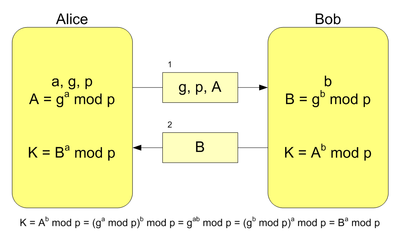
\includegraphics[scale=0.60]{Diffie.png} \end{center}
	\caption{Funcionamiento del sistema Diffie-Hellman}
\end{figure}

\

\subsubsection{Seguridad}
Este protocolo es vulnerable al ataque "man in the middle"; el cual consiste en que un tercero se coloca en el medio del canal y hace creer a ambos que es el otro. De esta forma se podría acordar una clave con cada parte y servir de "enlace" entre los dos participantes. Para que este ataque sea funcional se necesita saber que método de cifrado simétrico se va a emplear. Ocultar el algoritmo de cifrado no cumple con el principio de Kerkckhoffs de que la efectividad de un sistema no debe depender de que su diseño permanezca en secreto por lo que conocer el sistema que se va a emplear se hace trivial.

\

Para evitar esto se puede emplear un protocolo de autenticación de las partes mediante por ejemplo TLS(Transport Layer Security).

\begin{figure}[h]
	\begin{center}
		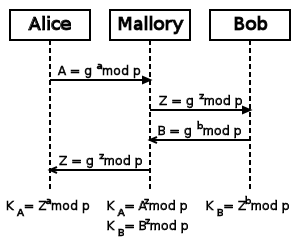
\includegraphics[scale=0.60]{man.png} \end{center}
	\caption{Esquema de la intrusión Man-in-the-middle}
\end{figure}



\subsection{\bf RC4}
\subsubsection{Concepto}
El algoritmo RC4 fue disenado por Ron Rivest en 1987 para la compañía RSA Data Security. Su implementación es extremadamente sencilla y rápida, y está orientado a  generar secuencias en unidades de un byte, ademas de permitir claves de diferentes  longitudes. Por desgracia es un algoritmo propietario, lo cual implica que no puede ser incluido en aplicaciones de tipo comercial sin pagar los royalties correspondientes.Su nombre completo es Rivest Cipher 4, teniendo el acrónimo RC un significado alternativo al de Ron's Code utilizado para los algoritmos de cifrado RC2, RC5 y RC6.

\

Inicialmente el algoritmo era un secreto registrado, pero en septiembre de 1994 una descripción del algoritmo fue posteada anónimanente en una lista de correo de Cypherpunks. Enseguida pasó al grupo de correo sci.crypt y de ahí fue publicado en numerosos sitios de Internet. Debido al conocimiento del algoritmo, éste dejó de ser un secreto registrado.

\

RC4 se ha convertido en parte de algunos protocolos y normas de cifrado de uso común, como WEP y WPA para tarjetas inalámbricas y TLS. Los principales factores en el éxito de RC4 sobre una amplia gama de aplicaciones tales son su velocidad y simplicidad, implementaciones eficientes en software y hardware son muy fáciles de desarrollar.

\subsubsection{Cifrado}

El cifrado RC4 esta basado en dos algoritmos. El primero es Key Scheduling Algorithm (KSA) y el segundo es Pseudo-Random Generation Algorithm (PRGA).

\

El algoritmo consta de una S-Caja de 8*8. Primero, el S-box array es llenado con valores secuenciales desde 0-255. Este array será llamado simplemente S. Entonces, el otro array de 256-bits es llenado con el valor de la "semilla" (clave), repitiendo como sea necesario hasta que todo el array es llenado. Este array es llamado K, y se mezcla el array K de la siguiente manera: 

\begin{itemize}
	\item \textbf{Key Scheduling Algorithm (KSA)}
	
	\
	
	\textbf{Inicialización:}\\
		$
		j=0;\\
		for\ i\ =\ 0\ to\ 255\\
		\{\\
		j\ =\ (j+S[i]\ +\ K[i])\ mod\ 256;$\\
		$intercambia\ S[i]\ y\ S[j];\\
		\}\\
		$
	\
	
	Cuando terminamos con esto, la S-box es intercambiada basándose en el valor de la "semilla". Esa es la "Key" programada para el uso en el algoritmo.
	
	\
	
	\item \textbf{Pseudo-Random Generation Algorithm (PRGA).}
	
	\
	
	\textbf{Generación de secuencia cifrante:}\\
	Ahora cuando se necesita el keystream data, que nos ayudara a cifrar y descifrar el mensaje, se usa el Pseudo-Random Generation Algorithm (PRGA). Este algoritmo tiene 2 contadores, el i y la j, en el cual ambos son inicializados en 0 para comenzar. Después de eso, cada bit de keystream data es usado en el siguiente Pseudo-Code:
	
	\
	
	$
	i\ =\ (i\ +\ 1)\ mod\ 256;\\
	j\ =\ (j\ +\ S[i])\ mod\ 256;\\
	intercambia\ S[i]\ and\ S[j];\\
	t\ =\ (S[i]\ +\ S[j])\ mod\ 256;\\
	Exponer\ valor\ de\ S[t];\\
	$
	
	
	El algoritmo RC4, genera una clave de flujo la cual es simplemente pasada por
	la función XOR para producir el flujo cifrado. Para descifrar se utiliza
	exactamente la misma función de cifrado. Una de las razones a las que
	debe su popularidad es su sencillez.	
\end{itemize}

\subsubsection{Ejemplo de RC4}
Para este ejemplo utilizaremos el texto original “HI” y lo veremos en binario.

\

H \\
0100 1000\\ 
XOR 0000 0011\\ 
--------------- \\
0100 1011 

\

I \\
0100 1001 \\
XOR 0000 0000\\ 
---------------- \\ 
0100 1001 

\

Texto original: 0100 1000 0100 1001\\
Texto cifrado: 0100 1011 0100 1001	

\

\subsubsection{Seguridad de RC4}
\begin{itemize}
	\item Algunos estudios indican que pueden existir claves débiles y que es sensible a estudios analíticos del contenido de la S- Caja. De hecho, algunos afirman que en una de cada 256 claves posibles, los bytes que se generan tienen una fuerte correlación con un subconjunto de los bytes de la clave.

	\item Se puede recuperar la clave empleada si la inicialización del algoritmo cumple determinadas premisas muy comunes, y se interceptan el suficiente número de mensajes. 

\end{itemize}

\

\subsubsection{Ventajas}

\begin{enumerate}
	\item Genera secuencias con periodos bastante grandes.
	\item Es inmune a los criptoanálisis diferencial y lineal.
	
	\item RC4 es uno de los cifradores más rápidos utilizados en aplicaciones serias y comerciales, siendo un cifrador de flujo, y como tal es básicamente un generador de números pseudo aleatorios inicializado desde una llave secreta por arriba de los 256 bytes (para el caso de ssl y para evitar el ataque Fluhrer, Martin,Shamir).	
\end{enumerate}	
\subsection{\bf Secure Hash Algorithm (SHA)}
\subsubsection{Concepto}
Los algoritmos hash se utilizan como componentes de otros algoritmos y procesos criptográficos para proporcionar servicios de seguridad de la información. Las funciones hash se utilizan a menudo con la fotografía digital Algoritmos de firma, códigos de autenticación de mensajes-clave hash, funciones de derivación de claves, y generadores de números aleatorios. Un algoritmo de hash convierte un mensaje de longitud variable en  una representación condensada de los datos electrónicos en el mensaje. Esta representación, o resumen del mensaje, se puede utilizar para las firmas digitales, la autenticación de mensajes, y otras aplicaciones seguras. Cuando se emplea en una aplicación de firma digital, el valor de hash del mensaje se firma en lugar del mensaje en sí mismo; el receptor puede usar la firma a verificar el firmante del mensaje y para autenticar la integridad del mensaje firmado.\cite{f}

\

Los algoritmos hash seguras son componentes del Kit de herramientas de cifrado del NIST que ayuda organizaciones federales y del sector privado seleccionar los componentes de seguridad criptográfica y procesos para proteger sus datos, comunicaciones y operaciones. 

\

Una función de hash seguro es una función resistente a colisiones, de una sola vía. Resistencia a la colisión significa que es muy difícil encontrar dos mensajes diferentes que producirán el mismo valor hash. Una forma significa que es fácil de calcular el valor hash de la entrada, pero es extremadamente difícil de reproducir la entrada desde el valor de hash, o encontrar otro de entrada que va a producir el mismo valor hash. Las funciones hash se utilizan a menudo para determinar si los datos han cambiado.

\

\subsubsection{Funciones Hash}

En una función HASH dicho valor será generado por una función H de la forma: $h=H (M)$

\

Donde:\\
M: Es una longitud variable del mensaje. \\
H(M): Es un valor HASH de longitud finita.

\

El valor HASH es aparentemente para el mensaje de la fuente de un tiempo cuando el mensaje es asumido o conocido que está correcto, donde el Receptor autentifica dicho mensaje pero recalcula el valor porque dicha función si no considera que el valor sea secreto.

\

Mensaje = M (Función Resumen = h (M) \\
Firma (rúbrica): r = EdE {h(M)} \\
dE : Es la clave privada del emisor que firmará h(M) \\

\subsubsection{SHA-0 y SHA-1}
SHA-1 forma parte de varias aplicaciones y protocolos de seguridad ampliamente utilizados, incluyendo TLS y SSL, PGP, SSH, S / MIME , y IPsec. Esas aplicaciones también pueden utilizar MD5 ; tanto MD5 y SHA-1 son descendientes de la MD4 . Hash SHA-1 también se utiliza en control de versiones distribuidos sistemas como Git, Mercurial, y monótono para identificar las revisiones, y para detectar la corrupción de datos o la manipulación. El algoritmo también se ha utilizado en la de Nintendo de Wii consola de juegos para la verificación de la firma cuando el arranque, pero un defecto significativo en las primeras implementaciones del firmware permite a un atacante eludir esquema de seguridad del sistema.


\begin{figure}[h]
	\centering
	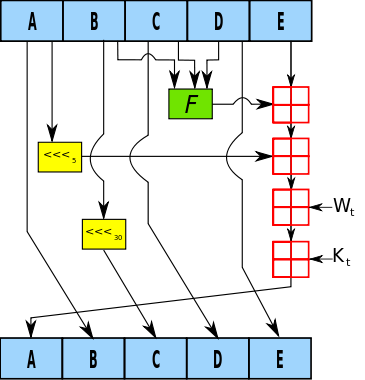
\includegraphics[scale=0.5]{imagen_1.png} 
	\caption{Representación gráfica de del SHA Básico}
\end{figure}

A, B, C, D y E son de 32 bits palabras de estado; F es una función no lineal que varía; n denota una rotación de la broca izquierda por n lugares; n varía para cada operación; W t es el mensaje de la palabra ampliada de ronda t; K t es la constante ronda de ronda t; denota adición módulo $2^23$.

\

Ejemplo:
Estos ejemplos son de SHA-1 resúmenes de mensajes en formato hexadecimal y en base 64 binario a ASCII codificación de texto.

\

SHA1 (El rápido zorro marrón salta sobre el perezoso dog) da hexadecimal:\\
2fd4e1c67a2d28fced849ee1bb76e7391b93eb12\\
en base 64 binario a ASCII de codificación de texto:\\
L9ThxnotKPzthJ7hu3bnORuT6xI

\

\subsubsection{SHA-2}

SHA-2 incluye cambios significativos respecto a su predecesor, SHA-1 . La familia SHA-2 consta de seis funciones hash con digestiones (valores hash) que son 224, 256, 384 o 512 bits: SHA-224, SHA-256, SHA-384, SHA-512, SHA-512/224, SHA -512 / 256 .

\begin{figure}[h]
	\centering
	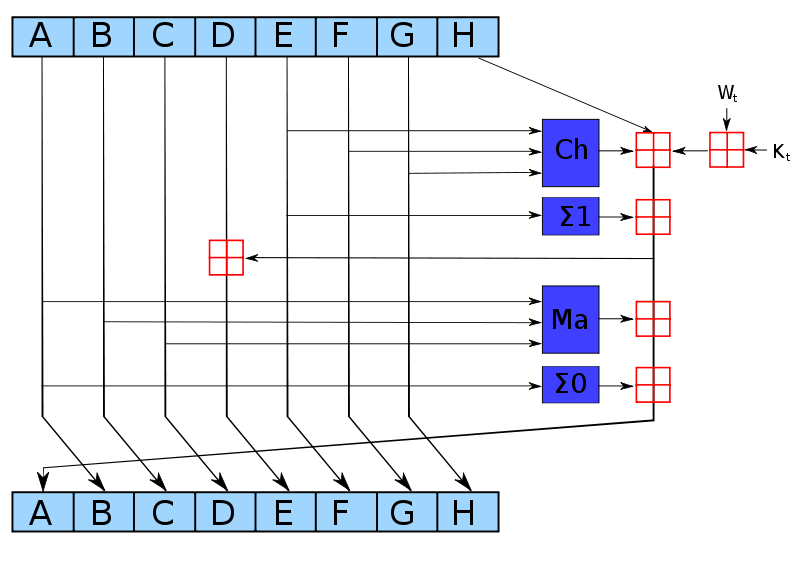
\includegraphics[scale=0.3]{imagen_2.png} 
	\caption{Representación gráfica de del SHA-2}
\end{figure}

\textbf{Aplicaciones}
La función hash SHA-2 se lleva a cabo en algunas aplicaciones y protocolos de seguridad ampliamente utilizados, incluyendo TLS y SSL , PGP , SSH , S / MIME , y IPsec.


\subsubsection{SHA-3}

La construcción de la esponja para las funciones de hash. P i son de entrada, z i son ordenadas de salida. El inusitado "capacidad" c debe ser el doble de la resistencia deseada a la colisión o ataques imagen inversa.

\

SHA-3 utiliza la construcción de esponja, en el que se "absorbe" los datos en la esponja, entonces el resultado es "exprimido" hacia fuera. En la fase de absorción, bloques de mensaje se XOR en un subconjunto del estado, que luego se transforma en su conjunto. En la fase de "squeeze", los bloques de salida se leen desde el mismo subconjunto del estado, alternadas con las transformaciones del Estado. El tamaño, r, de la parte del estado que se escribe y se lee que se llama la "tasa", y el sitio, c de la parte que está al margen de entrada / salida se denomina la "capacidad". La capacidad determina la seguridad del esquema. El nivel de seguridad máximo es la mitad de la capacidad.

\

En SHA-3, el estado consiste en un 5 x 5 matriz de palabras de 64 bits, 1600 bits en total. Keccak también se define para pequeños tamaños de palabra potencias de 2 W por debajo de 1 bit (25 bits en total estado). Tamaños pequeño estado pueden ser utilizados para probar los ataques criptoanalíticas y tamaños estado intermedio $ de w = 8 , 200 bits, para w = 32 , 800 bits $ se puede utilizar en aplicaciones prácticas, de peso ligero. 

\

La transformación de un bloque es una permutación que utiliza xor, y  no operaciones, y diseñado para una fácil implementación en software y hardware. Los autores afirman 12.5 ciclos por byte en un 2 Intel Core CPU. Sin embargo, en implementaciones de hardware, es notablemente más rápido que todos los demás finalistas. 

\begin{figure}[h]
	\centering
	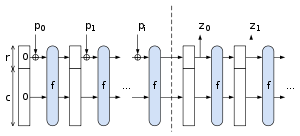
\includegraphics[scale=0.85]{imagen_4.png} 
	\caption{La construcción de la esponja para el hash.}
\end{figure}
$Pi$ son de entrada, $Zi$ son ordenadas de salida. El inusitado "capacidad" c debe ser el doble de la resistencia deseada a la colisión o ataques imagen inversa.

\bigskip\bigskip\bigskip\bigskip\bigskip

\pagebreak
\subsection{\bf Criptografía Cuántica}
\subsubsection{Concepto}
\subsubsection{Mecánica Cuántica en Criptografía}
\begin{itemize}
	\item Principio de Incertidumbre. 
	\item Polarizacion de un Foton.
	\item Qubits.\cite{Papa05}	
	\item Verschrankung
	\item Teorema de no-clonacion.
\end{itemize} \cite{i}\cite{j}\cite{Papa01}

\subsubsection{Distribucion de Claves Cuanticas}
\cite{Papa06}Se deben cumplir las siguientes condiciones:

\

\begin{itemize}
	\item Ningun intruso puede obtener la clave transmitida 
	\item Cualquier intento de intromisión para obtener la clave transmitida puede ser detectado con alta probabilidad
	\item Los usuarios pueden estar seguros de que están compartiendo la misma clave
\end{itemize}

\

\subsubsection{Protocolo BB84}
El esquema propuesto en 1984 por Brassard y Bennett implica el envío de fotones preparados en diferentes estados de polarización.\cite{Papa02}\cite{Papa09}


\begin{figure}[hbtp]
	\centering
	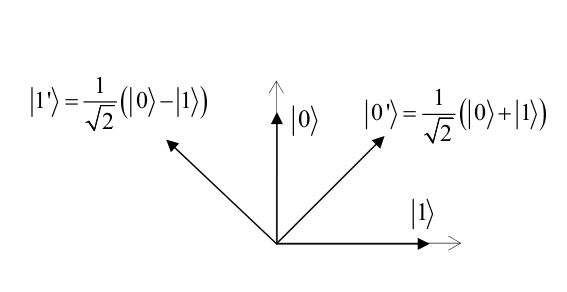
\includegraphics[scale=0.4]{1.png} 
	\caption{Polarizacion de fotones en el protocolo BB84.}
\end{figure}

Usando un filtro de polarización, se selecciona el ángulo de polarización con respecto a la horizontal. También se puede usar un método más sofisticado, en el que se usa un aparato conocido como Pockels cell que hace posible que el campo eléctrico del fotón oscile en el plano deseado. Como se vio anteriormente, se pueden elegir cuatro ángulos en particular: 0, 45, 90, y 135 grados, $\leftrightarrow \nearrow \updownarrow \searrow$. Los fotones polarizados en ángulos de 0 y 45 representan el valor binario 0, y los fotones polarizados en ángulos de 90 y 135 representan el valor binario 1; una vez hecha esta
correspondencia, una secuencia de bits puede ser convertida en una secuencia de fotones polarizados.

\pagebreak

{\bf 1. Sin la Presencia de Eve.- }
\begin{itemize}
	\item Alicia codifica bits como fotones polarizados. La primera fila indica la secuencia de bits. La segunda indica la orientación usada por el filtro. La tercera indica el resultado de la polarización.\cite{Papa03}
	
	\begin{figure}[hbtp]
		\centering
		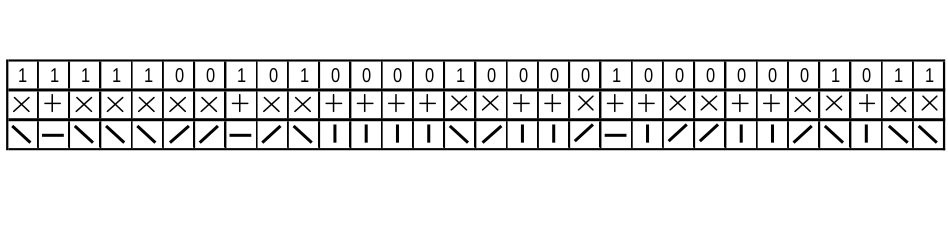
\includegraphics[scale=0.22]{2.png} 
		\caption{Alice codifica bits como fotones polarizados}
	\end{figure}
	
	Alicia genera una secuencia de fotones. Cuando Bob recibe los fotones, decide aleatoriamente si medir las polarizaciones a lo largo de las direcciones rectilíneas o a lo largo de las diagonales. De esta forma Bob podría extraer un bit de información por cada fotón.
	
	\item Bob decodifica fotones polarizados como bits. La primera fila indica la secuencia de fotones recibida. La segunda fila indica la configuración del cristal de calcita de Bob. La tercera fila indica el resultado de la medición.
	
	\begin{figure}[h]
		\centering
		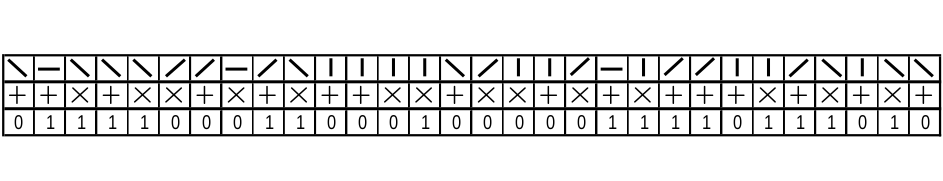
\includegraphics[scale=0.22]{3.png} 
		\caption{Bob decodifica fotones polarizados como bits}
	\end{figure}
	
	Este comportamiento se explica por el principio de incertidumbre de Heisenberg.
	\begin{figure}[h]
		\centering
		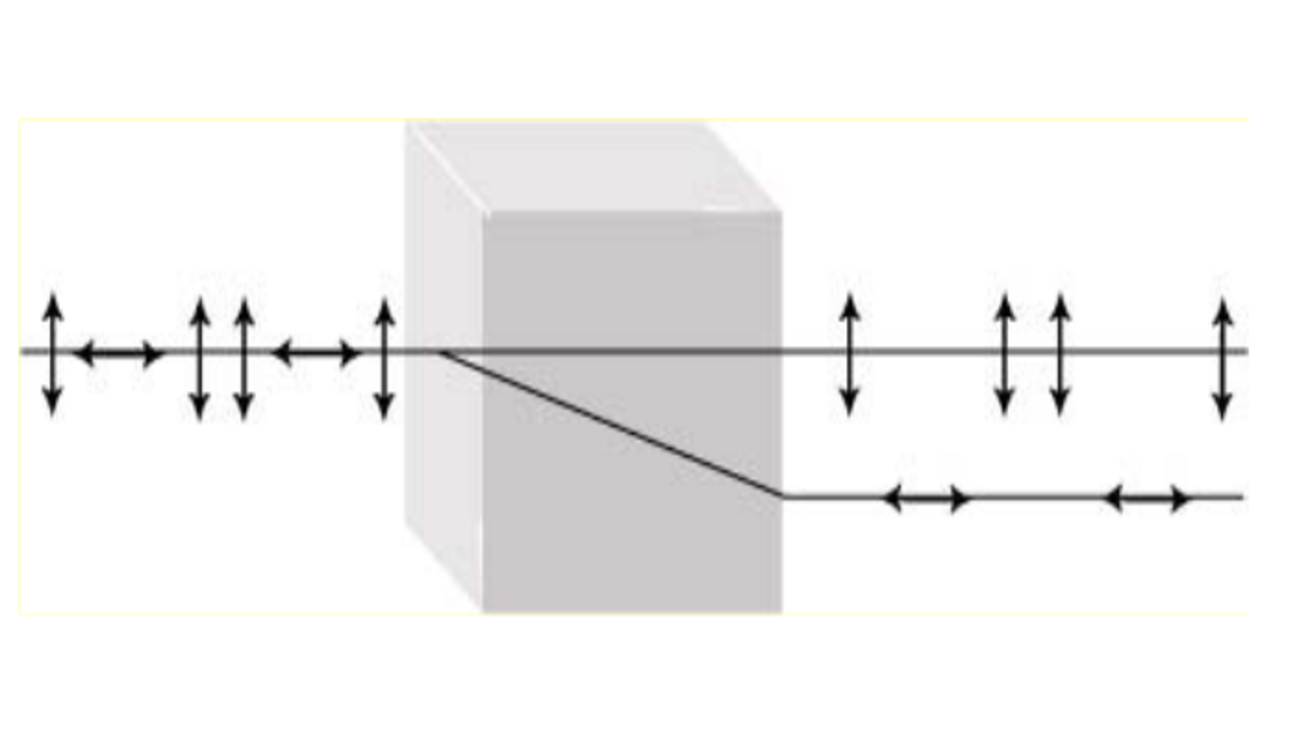
\includegraphics[scale=0.15]{4.png} 
		\caption{Cristal de Calcita que separa fotones.}
	\end{figure}
	
	Alicia le dice a Bob (canal clasico) el valor de los bits que debió haber medido, y la verificación debe asegurar que los bits de Bob concuerdan al 100\% con los de Alicia.
	
	La probabilidad de detectar un espía que esté presente es $1-\left(\frac{3}{4}\right)^{N}$.
	
	\item Alicia y Bob comparan un subgrupo de bits para probar, y verificar la presencia de un espía. En todos los bits se usó la misma orientación para polarizar y medir, y el valor del bit es igual, mostrando que no hay un espía presente.
	
	\begin{figure}[hbtp]
		\centering
		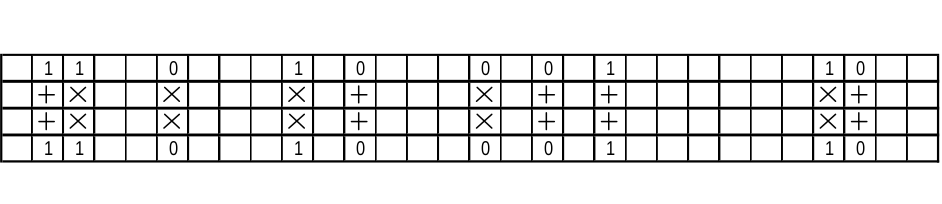
\includegraphics[scale=0.22]{5.png} 
		\caption{Alicia y Bob comparan un subgrupo de bits}
	\end{figure}
	
	\item Clave generada. Los casos en que la orientación del polarizador es igual a la orientación del cristal, se representan por :), y esto significa que el bit se tomó como parte de la clave.
	
	\begin{figure}[hbtp]
		\centering
		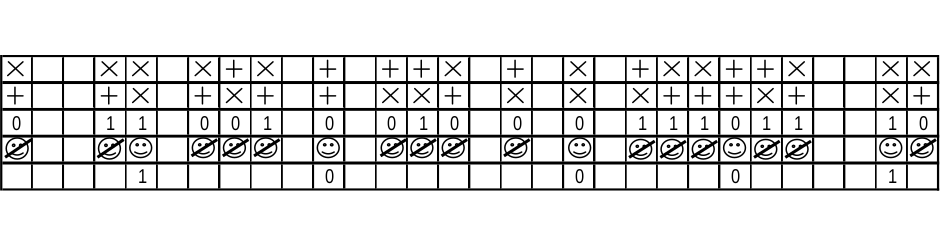
\includegraphics[scale=0.22]{6.png} 
		\caption{Clave Generada}
	\end{figure}
	
\end{itemize}

{\bf 2. Eve Presente.- } En este caso, para que Eva pueda medir los fotones interceptados, debe haber escogido una orientación de polarización. Si Eva quisiera tener certeza de no ser detectada, necesitaría correr la suerte de escoger para cada bit transmitido la misma orientación de polarización que Alicia, lo cual, si el tamaño de la clave es lo suficientemente largo, sería prácticamente imposible. Si Eva elige la orientación incorrecta, modificará la polarización del fotón y su presencia podrá ser detectada en la fase de prueba.\cite{Papa04}

\begin{itemize}
	\item Codificación de los bits de Alicia a estados de polarización:
	
	\begin{figure}[hbtp]
		\centering
		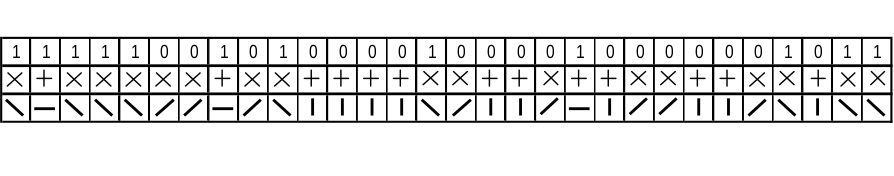
\includegraphics[scale=0.22]{7.png} 
		\caption{Codificación de los bits de Alicia}
	\end{figure}
	\item Intercepción y medición de Eva (Si las polarizaciones no son iguales, Eva modifica irreparablemente el estado original):
	
	\begin{figure}[hbtp]
		\centering
		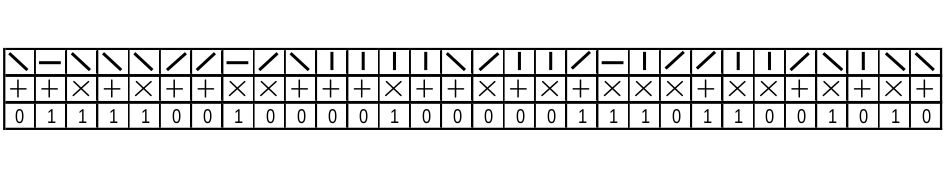
\includegraphics[scale=0.22]{8.png} 
		\caption{Intercepción y medición de Eva}
	\end{figure}
	\pagebreak
	\item Bob, aún sin estar consciente de la presencia de Eva, realiza sus mediciones:
	
	\begin{figure}[hbtp]
		\centering
		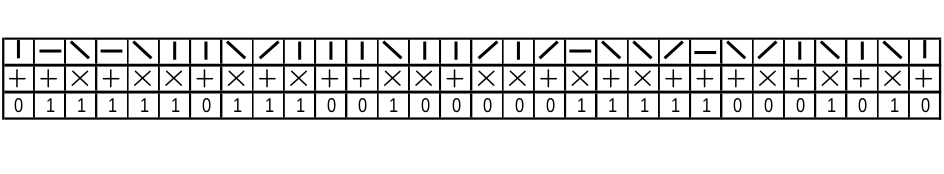
\includegraphics[scale=0.22]{9.png} 
		\caption{Bob realiza mediciones}
	\end{figure}
	
	\item Pero en la fase de prueba, Alicia y Bob detectan la presencia de Eva y deciden desechar toda la secuencia de fotones para empezar de nuevo el procedimiento.
	
	\begin{figure}[hbtp]
		\centering
		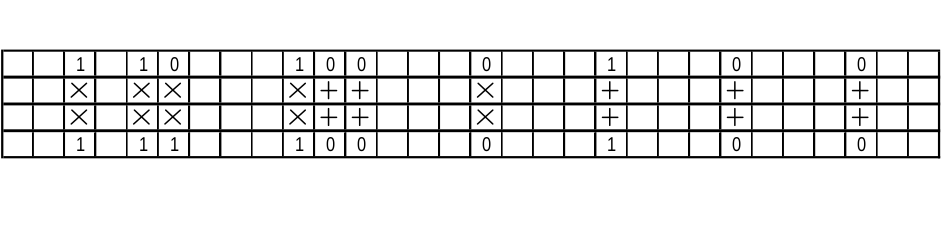
\includegraphics[scale=0.22]{10.png} 
		\caption{Detectan la presencia de Eva}
	\end{figure}
\end{itemize}

\subsection{\bf Advanced Encryption Standard (AES)}
\subsubsection{Concepto}
 Este algoritmo (también llamado, Rijndael por sus creadores Joan Daemen y Vincent Rijmen) fue publicado por el NIST en 2001, el cual presenta diferencias notable con respecto al resto de los cifradores simétricos, entre ellos destacan de manera sobresaliente: el tamaño de los bloques de 128 bits, manejo de claves de longitudes diferentes y uso de matemáticas polinomiales en estructuras de campos finitos.\cite{a}

\

AES presenta dos características importantes:

\

\begin{enumerate}
	\item \textbf{Linealidad:} El algoritmo debe probar que no existe linealidad o correlación alguna entre las entradas y las salidas, dicho de otra manera, que las salidas no sean una función directa de las entradas, y no haya posibilidad de determinar alguna dependencia entre los datos de entrada y los que salen. Para ello el algoritmo debe considerar la alternancia de claves, de ahí la importancia de utilizar una clave distinta en cada iteración.
	\pagebreak
	\item \textbf{Propagación:} El algoritmo debe realizar una adecuada propagación de las diferencias de los bits, de manera que haya una alta dispersión de los bits en el mensaje de cifrado y no sean identificados en un ataque criptoanalista. Así, una buena propagación será capaz de bloquear un criptoanálisis diferencial ya que posibilitará derivar información de la clave a partir de conocer las probabilidades de las diferencias de la propagaciórn, por lo tanto, debe buscarse que estas probabilidades sean muy pequeñas y para ello, entre otros aspectos resulta relevante la cantidad de iteraciones que se deben realizar.
\end{enumerate}

\

\subsubsection{Proceso de creación del AES}

\begin{figure}[h]
	\centering
	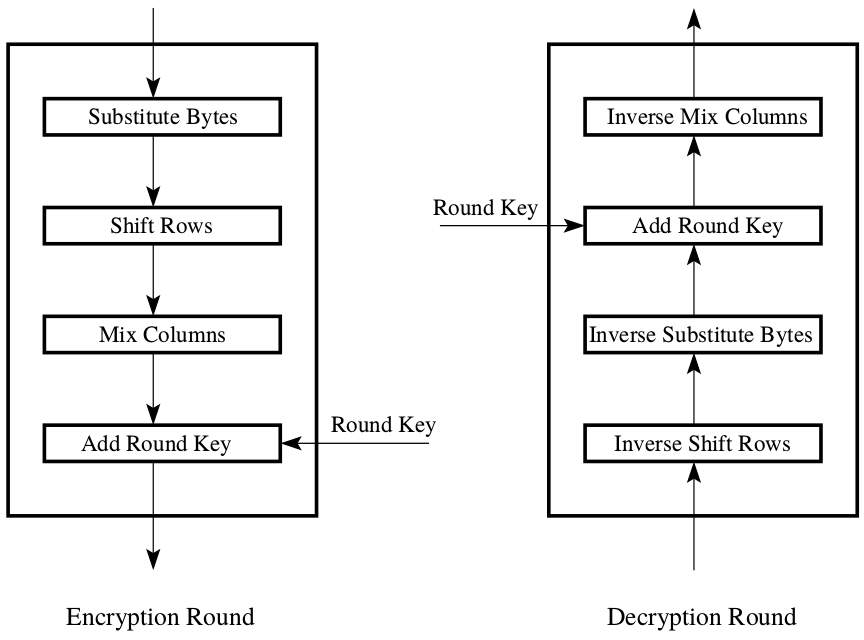
\includegraphics[scale=0.28]{aes_main.png} 
	\caption{Gráfico de la encriptacion y desencriptacion con AES}
\end{figure}

\begin{enumerate}
	\item \textbf{SubBytes} es una sustitución de byte por byte que se realiza durante todo el proceso.
	
	\begin{itemize}
		\item Este paso consiste de usar una tabla de 16 x 16 para encontrar un byte de reemplazo para un byte dado en la matriz de entrada.
		\item Las entradas de la tabla de búsqueda se crean mediante el uso de las nociones
		de inversos multiplicativos en GF ( $2^8$ ) y la aleatorización de bits de
		destruir las correlaciones a nivel de bits dentro de cada byte .
	\end{itemize}
	\item \textbf{ShiftRows} se usa para desplazar las filas de una matriz durante el proceso hacia adelante.
	\begin{itemize}
		\item El objetivo de esta transformación es que revolver el orden de bytes
		dentro de cada bloque de 128 bits
	\end{itemize}
	
	\begin{figure}[h]
		\centering
		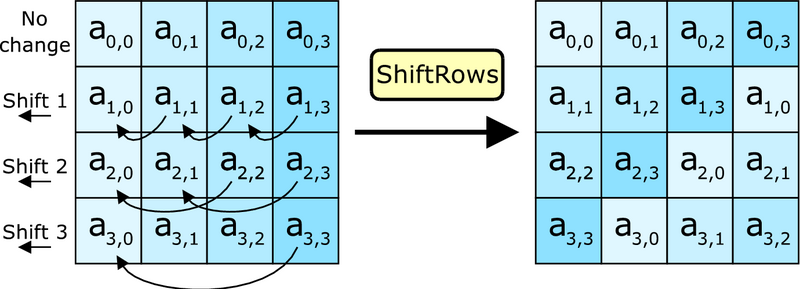
\includegraphics[scale=0.25]{ShiftRows.png} 
		\caption{ShiftRows haciendo una que las filas se desplacen.}
	\end{figure}
	\pagebreak
	\item \textbf{MixColumns} hace la mezcla de los bytes en cada columna por separado durante el proceso hacia adelante.
	
	\begin{figure}[h]
		\centering
		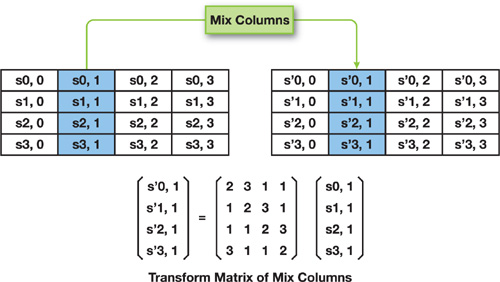
\includegraphics[scale=0.6]{MixColumns.jpg} 
		\caption{MixColumns haciendo una Multiplicacion de columnas.}
	\end{figure}
	
	\item \textbf{AddRoundKey} cada byte del «state» es combinado con la clave «round»; cada clave «round» se deriva de la clave de cifrado usando una iteración de la clave.
	
	\begin{figure}[h]
		\centering
		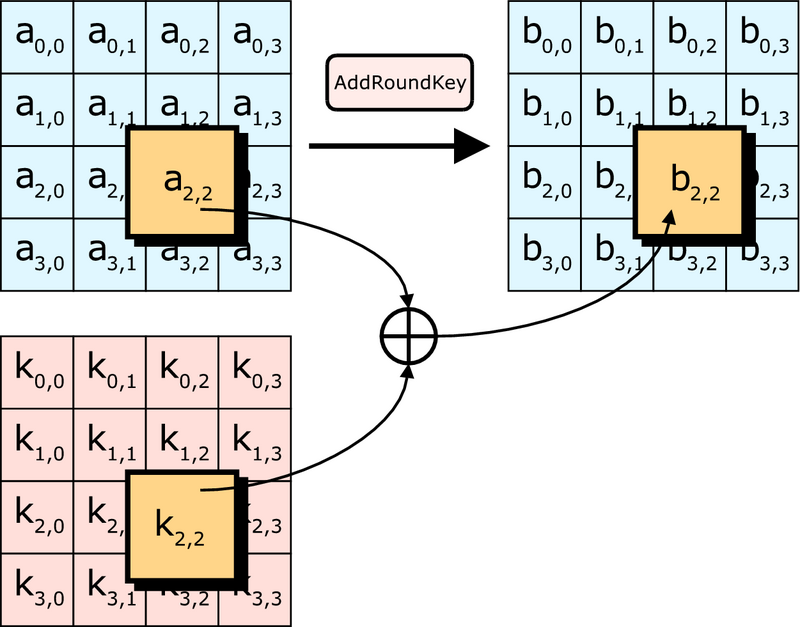
\includegraphics[scale=0.22]{AddRoundKey.png} 
		\caption{Ejemplo de AddRoundKey}
	\end{figure}
	
	En el paso AddRoundKey, cada byte del state se combina con un byte de la subclave usando la operación XOR.\cite{b}
\end{enumerate}

\
\pagebreak
\subsubsection{Seguridad}
El método más común de ataque hacia un cifrador por bloques consiste en intentar varios ataques sobre versiones del cifrador con un número menor de rondas. El AES tiene 10 rondas para llaves de 128 bits, 12 rondas para llaves de 192 bits, y 14 rondas para llaves de 256 bits. 

\

En 2002, un ataque teórico, denominado "ataque XSL", fue anunciado por Nicolas Courtois y Josef Pieprzyk, mostrando una potencial debilidad en el algoritmo AES. Varios expertos criptográficos han encontrado problemas en las matemáticas que hay por debajo del ataque propuesto, sugiriendo que los autores quizá hayan cometido un error en sus estimaciones. Si esta línea de ataque puede ser tomada contra AES, es una cuestión todavía abierta. Hasta el momento, el ataque XSL contra AES parece especulativo; es improbable que nadie pudiera llevar a cabo en la práctica este ataque.

\

Hasta 2005, no se ha encontrado ningún ataque exitoso contra el AES. La Agencia de Seguridad Nacional de los Estados Unidos (NSA) revisó todos los finalistas candidatos al AES, incluyendo el Rijndael, y declaró que todos ellos eran suficientemente seguros para su empleo en información no clasificada del gobierno de los Estados Unidos. En junio de 2003, el gobierno de los Estados Unidos anunció que el AES podía ser usado para información clasificada.

\section{Conclusión}
Esta investigación nos a demostrado que desde tiempos antiguos hemos vivido en una sociedad donde la criptografía a estado presente pero se ocultaban de nuestra vista.

La criptografía es y sera el método más utilizado para ocultar mensajes dentro de la guerra como en la zona computacional

\

El análisis de todas las clases de criptografía nos a hecho ver que no son eternas y que siempre se va a estar en constante creación de algoritmos de encriptación ya que tarde o temprano terminan rompiendo la encriptación.

\

Con respecto a nuestras investigaciones donde profundizamos en un tema en específico hemos podido ver que las matemáticas son la base indiscutible de la encriptación.
\bigskip\bigskip\bigskip\bigskip\bigskip
\bigskip\bigskip\bigskip\bigskip\bigskip
\bigskip\bigskip\bigskip\bigskip\bigskip

\pagebreak

\onecolumn

\bibliographystyle{plain}
\bibliography{biblio.bib}

\bigskip\bigskip\bigskip\bigskip\bigskip
\bigskip\bigskip\bigskip\bigskip


\pagebreak



\listoffigures


\end{document}